%DIJOUS
\newcommand{\refscreen}[1]{\hyperref[fig:montezuma-map]{screen~#1}}
\chapter{Methodology}
\section{\acl{MR}}
\subsection{Description\label{subsec:mr-description}}
You, the player, are Panama Joe, an intrepid explorer-archaeologist. Your latest
trip has brought you to discover the entrance to an Aztec pyramid. Filled with
excitement, you rush to search the treasures that surely await inside. But the
pyramid is full of traps and monsters. You will need all of your wits and agility to
get out alive!\footnote{Game background from the review by \citet{adair2007montezuma}.}

In the game, Panama Joe can run, jump and climb ladders, ropes and poles. The
pyramid he can explore is divided in 24 screens, numbered 0--23, depicted in
\ffref{fig:montezuma-map}. The player starts the game in screen 1 and ends when
collecting the gems in screen 15. When the player completes the game, it simply
resets with a different colour scheme.

Joe has a number of lives, initially 5. When they are over and Joe loses a life
again, the game is over. Lives can be lost by touching monsters, touching blue
wall traps (such as those in \refscreen{12}), falling
into quicksand pits or falling from too high.

The player can gain score for a number of things: collecting gems (+1000),
keys (+100), the sword (+100), the torch (+3000) or the mallet (+200); opening a
door (+300); or killing a monster with the sword (+2000). A life
is gained for every $10\,000$ points gained, with a maximum of 6 lives. The
torch allows you to see in the lowest floor of the pyramid (which is otherwise
black). The sword allows you to kill one monster. The mallet allows you to be
immune to monsters for a period of time.

The game can be rendered impossible to complete, since there are 6 doors but
only 4 keys. The two doors in \refscreen{17} need to be opened to finish, and
either one of the doors in \refscreen{1} needs to be opened to do almost
anything. So the player can either open both doors in \refscreen{1} and not see
in the bottom floor, or leave one door in each of the screens 1 and 4 unopened.

At each time step, the player can take 8 different actions: \textsc{Noop} (stay
still), \textsc{Fire} (jump straight up), \textsc{Up}, \textsc{Right},
\textsc{Left}, \textsc{Down}, \textsc{LeftFire} (jump to the left),
\textsc{RightFire}. The rest of the 18 actions permitted by the Atari overload
to one of these.

\begin{figure}[p]
\setlength{\unitlength}{\textwidth}
\begin{center}
%\noindent\makebox[\textwidth]{
  \begin{picture}(1,.513)
    \put(0,0){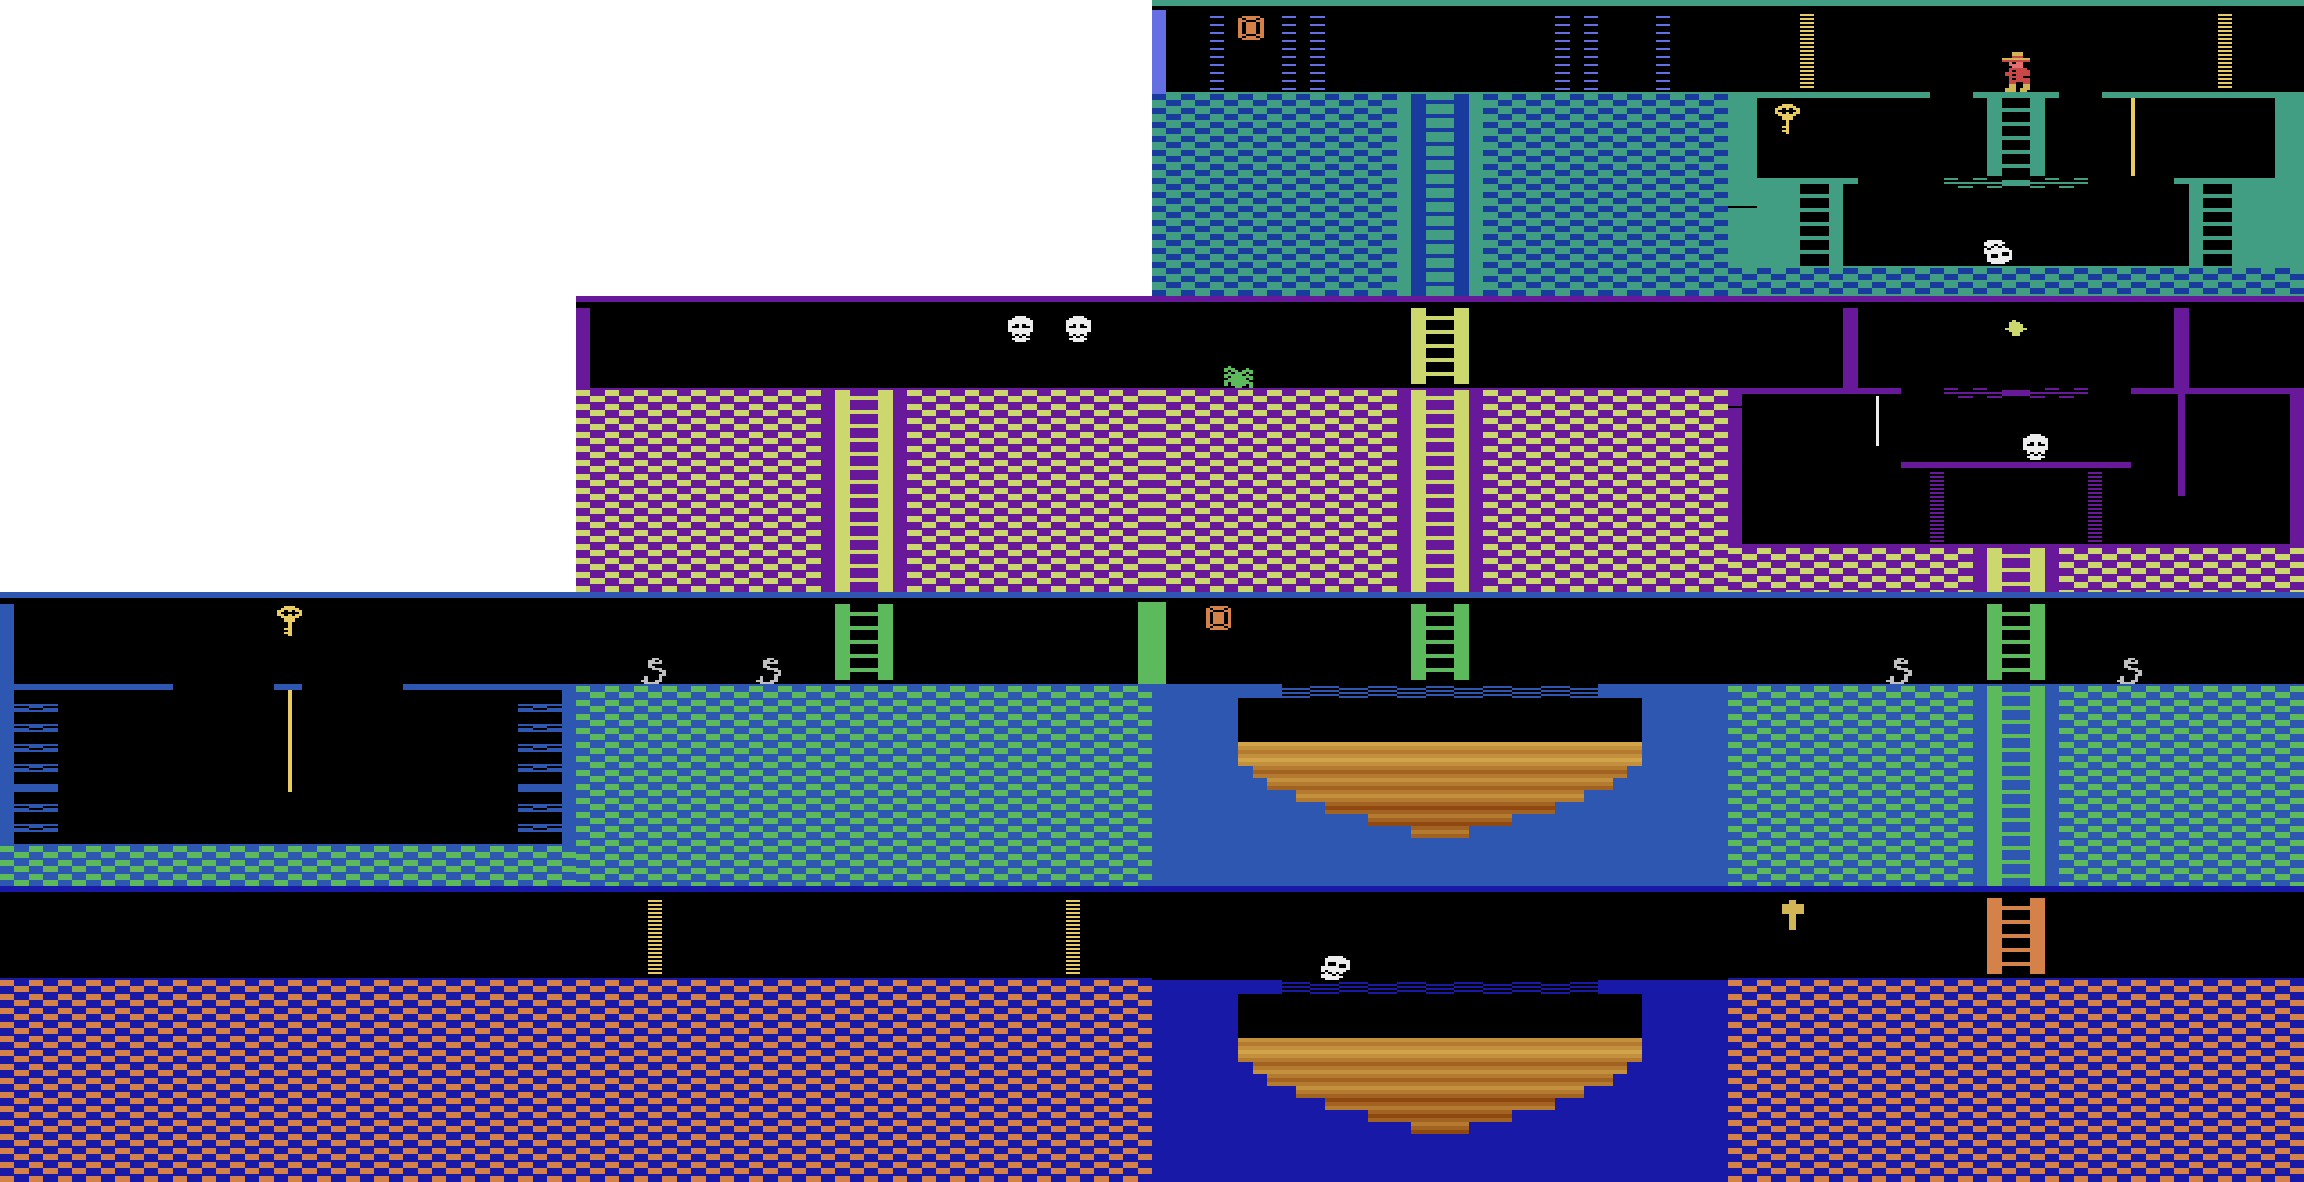
\includegraphics[width=\unitlength]{img/montezuma_all_pt1.png}}
    \put(.58,.485){\color[rgb]{1,1,1}\makebox(0,0)[lb]{0}}
    \put(.83,.485){\color[rgb]{1,1,1}\makebox(0,0)[lb]{1}}
    \put(.33,.357){\color[rgb]{1,1,1}\makebox(0,0)[lb]{3}}
    \put(.58,.357){\color[rgb]{1,1,1}\makebox(0,0)[lb]{4}}
    \put(.83,.357){\color[rgb]{1,1,1}\makebox(0,0)[lb]{5}}
    \put(.08,.228){\color[rgb]{1,1,1}\makebox(0,0)[lb]{8}}
    \put(.30,.228){\color[rgb]{1,1,1}\makebox(0,0)[lb]{9}}
    \put(.58,.228){\color[rgb]{1,1,1}\makebox(0,0)[lb]{10}}
    \put(.83,.228){\color[rgb]{1,1,1}\makebox(0,0)[lb]{11}}
    \put(.08,.1){\color[rgb]{1,1,1}\makebox(0,0)[lb]{16}}
    \put(.33,.1){\color[rgb]{1,1,1}\makebox(0,0)[lb]{17}}
    \put(.6,.1){\color[rgb]{1,1,1}\makebox(0,0)[lb]{18}}
    \put(.83,.1){\color[rgb]{1,1,1}\makebox(0,0)[lb]{19}}
  \end{picture}
%}

\vspace{.2cm}

%\noindent\makebox[\textwidth]{
  \begin{picture}(1,.513)
    \put(0,0){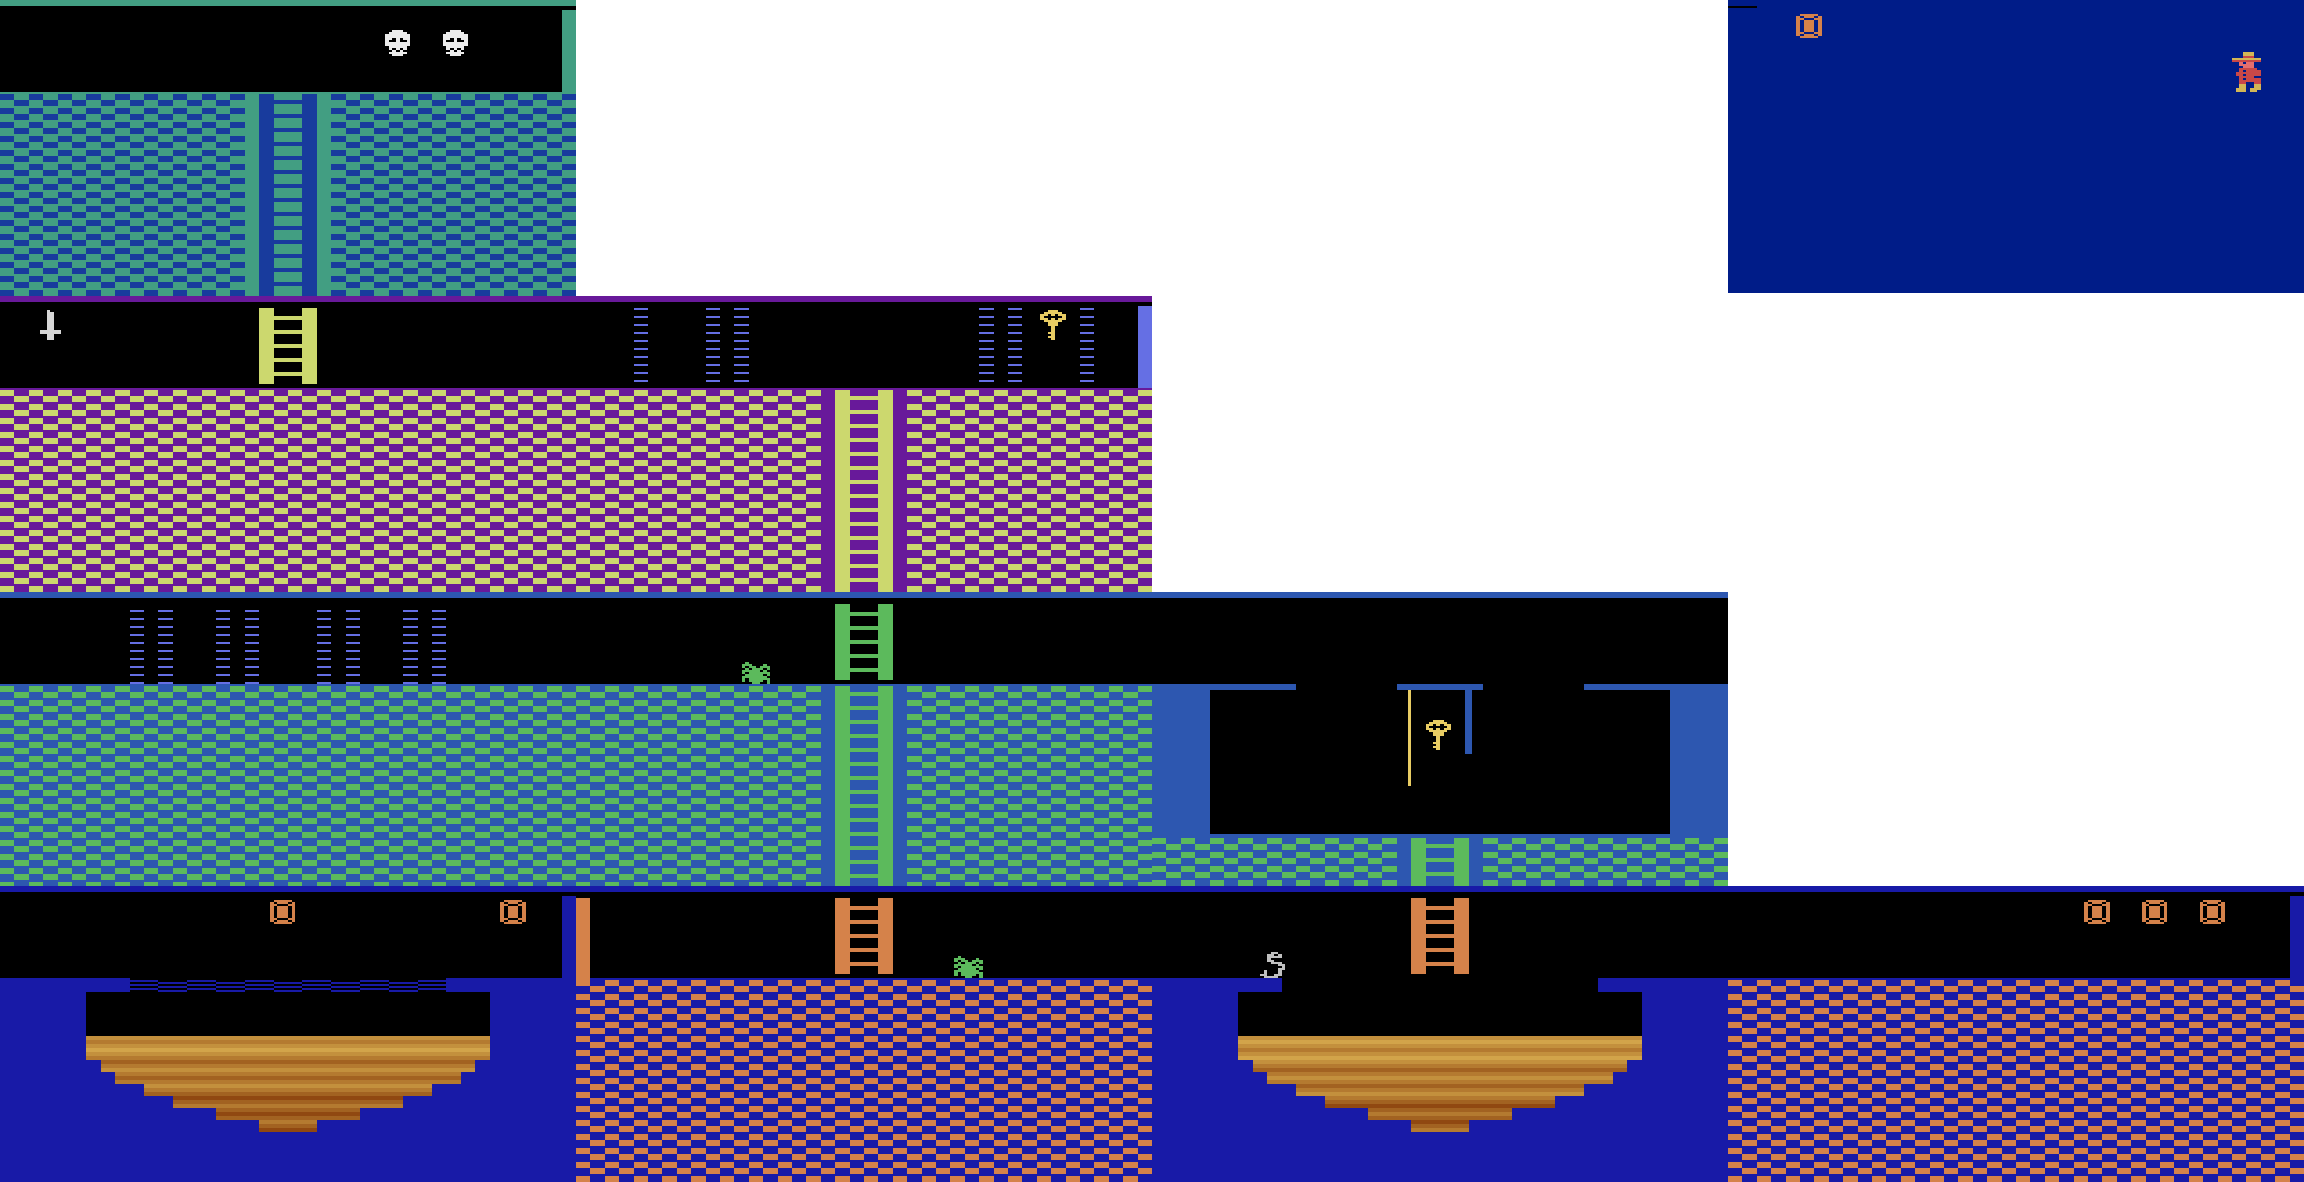
\includegraphics[width=\unitlength]{img/montezuma_all_pt2.png}}
    \put(.08,.485){\color[rgb]{1,1,1}\makebox(0,0)[lb]{2}}
    \put(.83,.485){\color[rgb]{1,1,1}\makebox(0,0)[lb]{15}}
    \put(.08,.357){\color[rgb]{1,1,1}\makebox(0,0)[lb]{6}}
    \put(.33,.357){\color[rgb]{1,1,1}\makebox(0,0)[lb]{7}}
    \put(.04,.228){\color[rgb]{1,1,1}\makebox(0,0)[lb]{12}}
    \put(.28,.228){\color[rgb]{1,1,1}\makebox(0,0)[lb]{13}}
    \put(.58,.228){\color[rgb]{1,1,1}\makebox(0,0)[lb]{14}}
    \put(.08,.1){\color[rgb]{1,1,1}\makebox(0,0)[lb]{20}}
    \put(.33,.1){\color[rgb]{1,1,1}\makebox(0,0)[lb]{21}}
    \put(.58,.1){\color[rgb]{1,1,1}\makebox(0,0)[lb]{22}}
    \put(.83,.1){\color[rgb]{1,1,1}\makebox(0,0)[lb]{23}}
  \end{picture}
%}
\end{center}
\caption[The complete map of \acl{MR}.]{The complete map of \acl{MR}. Rooms are
numbered from left to right and from top to bottom. The pyramid they form has
been cut to fit in the page. Room 15 is located to the left of room 16. The
screens are not numbered in the game. The player starts in room 1 and finishes
in room 15.\label{fig:montezuma-map}}
\end{figure}

\subsection{Memory layout of the Atari 2600}
The Atari 2600 uses the 6507 \ac{CPU}, which can address $8\,$KB of memory.
Addresses range from 0x0000 to 0x1FFF. Addresses larger than 0x1000, included,
are mapped to the \ac{ROM} cartridge that contains the code of the game.
Addresses lower than that are used for drawing to screen, looking at the
controller input, \dots and, most importantly, the \ac{RAM}. The 2600 has only
128 bytes of \ac{RAM}, which are addressed in the range 0x0080--0x00FF, both
included. \citep{atarispec}

Throughout this document we will prefix a number with ``0x'' if it is expressed
in base 16. If a described memory position has four hexadecimal digits, it is an
absolute processor address. Otherwise, it is assumed to be in the range
0x0000--0x00FF.


\subsection{Reverse-engineering \acl{MR}\label{subsec:rev-eng-mr}}
We used the \acl{ALE} (\cite{bellemare2013arcade}) to take several simultaneous
screen and \ac{RAM} snapshots. We usually took 5 to 10 snapshots in the space of
1 or 2 seconds, while performing certain action in the game. Then, we looked at
the bytes that changed value from snapshot to snapshot.

We also used the debugger built-in to the Atari 2600 emulator, Stella
(\cite{stella}). Using the command \verb-breakif <condition>-, that pauses the
game and shows the debugger if a condition is met, enabled us to play and check
whether a memory position behaved as we suspected. In some cases we used the
disassembled code in that debugger too.

In \ffref{tab:atari-ram} and in the list below we reproduce the layout of
the Atari 2600's main memory and what each position affects in \acl{MR}.

Some entries can be modified in the Stella debugger when the game is running,
and affect the game. If an entry is not editable, it will be marked with an
asterisk (*). The values that are not marked editable may be editable in other
circumstances, and are probably editable in the middle of the computations
within a frame. However, their value has been observed only going back to what
it was if modified between frames.

We have a very strong suspicion that nowhere in the \ac{RAM} is stored the
layout of the screen, or where collisions can occur. This is coded into the
programming path (with branches depending on the character's position), or
stored somewhere in the ROM. A learner that hopes to generalise between screens
needs to have access to that information.

\begin{table}[hbtp]
\begin{center}
\newcommand{\ram}[2]{\hyperref[ram:#1]{#2*}}
\newcommand{\rame}[2]{\hyperref[ram:#1]{#2}}
%\newcommand{\ram}[2]{\ref{ram:#1}*}
%\newcommand{\rame}[2]{\ref{ram:#1}}
\begin{tabular}{c|cccccccccccccccc}
  & 0 & 1 & 2 & 3 & 4 & 5 & 6 & 7 & 8 & 9 & A & B & C & D & E & F \\
\hline
8 &\rame{frame}{80}&   &   &\rame{screen}{83}&   &   &   &   &   &   &   &   &   &   &   &   \\
9 &   &   &   &\rame{score}{93}& \rame{score}{94}& \rame{score}{95}&   &   &   &   &   &   &   &   &\ram{player-sprite}{9E}&   \\
A &   &   &   &   &   &   &   &   &   &   &\rame{x}{AA}&\rame{y}{AB}&   &   &   &   \\
B &   &\rame{collectable}{B1}&\rame{collectable-colour}{B2}&  &\rame{look-lr}{B4}&  &   &   &   &   &   \rame{lives}{BA} & & & &\rame{skull-animation}{BE}&\rame{skull-jump-y}{BF}\\
C &   &\rame{inventory}{C1}&\ram{doors}{C2}&\rame{skull-moving}{C3}&   &   &   &   &   &   &   &   &   &   &\rame{skull-rotate-y}{AE}&\rame{skull-rotate-x}{AF}\\
D &   &   &   &   &\rame{sprite-modifier}{D4}&   &  \rame{jump}{D6}&   &\rame{fall}{D8}&   &   &   &   &   &  & \\
E &   &   &   &   &   &   &   &   &   &   &\ram{skull-n-rotations}{EA}&   &   &   &   &   \\
F &   &   &   &   &   &   &   &   &   &   &   &   &   &   &   &   \\
\end{tabular}

\end{center}
\caption{The known \acs{RAM} layout for \acl{MR}.\label{tab:atari-ram}}
\end{table}

{
\newcommand{\entry}[2]{\item\label{ram:#1}\textbf{0x#2}: Not editable.}
\newcommand{\entrye}[2]{\item\label{ram:#1}\textbf{0x#2}: Editable.}
\newcommand{\n}[1]{0x#1}

\begin{enumerate}
\entrye{lives}{BA} The number of lives the player has left, that is, the number of
times the player can die and continue the game afterwards. Controls the number
of hats displayed at the top. Panama Joe starts with 5 lives. The counter can go
up to 6 without graphical problems.

\entrye{screen}{83} The current screen. If edited, the new screen will only be
partially drawn. Sometimes, one can exit the screen and reenter it by playing
and the issue will go away.

\entrye{x}{AA} The X position of the character. If set to the middle of the air,
Panama Joe will fall.

\entrye{y}{AB} The Y position of the character. If set to the middle of the air,
and there is a platform below, the character will not fall! Instead, it will
behave as if it was on a ladder. The Y values of the three floors that every
level has are \n{94} or \n{9C}, \n{C0}, and \n{EB}.

\entrye{jump}{D6} The current frame of the jump. Set to \n{FF} when in the
ground. Set to \n{13} when the jump starts. When jumping, the game adds to the Y
of Panama Joe the values from the array starting at memory position \n{1E47}.
Thus, if set to higher than \n{13}, the game behaves oddly. It also can be reset
to whatever value at any time, causing Panama Joe to start a jump, even in
mid-air.

\entrye{fall}{D8} The current frame of the fall. Normally set to \n{00}. When falling
off an elevated ground, or off a jump, this value will begin to count up. If it
is \n{08} or higher when Panama Joe touches the ground, he will die.

\item\label{ram:score}\textbf{0x93}, \textbf{0x94}, \textbf{0x95}: Editable. The
score, represented in \acl{BCD}. This is, every nibble represents a decimal digit.

\entrye{inventory}{C1} The contents of the player's inventory. Each possible
object in it is associated to a bit, that is set if the object is in the
inventory. At most 6 objects can be carried without causing graphical
corruptions. The objects and their associations are:
\begin{center}
\begin{tabular}{c|c|c|c|c|c|c|c}
\n{80} & \n{40} & \n{20} & \n{10} & \n{08} & \n{04} & \n{02} & \n{01} \\
\hline
torch & sword & sword & key & key & key & key & mallet \\
\end{tabular}
\end{center}
If the inventory's value is changed, collecting items by touching them stops
working.

\entry{doors}{C2 (bits 3, 2)} Whether the doors in the screen are closed or
open. Only means this in screens 1, 5 and 17. When the bit is set, the door is
closed. Bit 3 controls the door in the left, bit 2 the one in the right.

\entrye{frame}{80} The current frame. This memory position starts the game at
\n{00} and increments by one every frame.

\entrye{skull-animation}{BE} The frame of the rotating skull's animation, in
screens where there is one.

\entrye{skull-rotate-x}{AF} X of the rotating skull, when there is one (screens
1 and 18). It is not in the same scale as the player's X. Its values range from
0x16 to 0x48, inclusive.

\entrye{skull-rotate-y}{AE} Y of the rotating skull. Also in its own scale, and
cannot take it away from its floor.

\entry{skull-n-rotations}{EA} The number of times the rotating skull in the
first screen has changed direction. Remains even after changing screen. If
untouched, the lowest byte indicates the direction the skull is moving in. Can
be changed, but it does not change the direction of the skull.

\entrye{skull-jump-y}{BF} relative Y position of the jumping skulls, in screens where they are present.
It oscillates between \n{00} and \n{0F}, where 0 is the topmost position. The
game makes relative changes to this value, so if set to F while the skulls on
mid-air, they will not go below that point afterwards.

\entrye{skull-moving}{C3 (bit 1)} Whether the rotating skull is moving (set) or
not (unset). The function of the rest is unknown.

\entry{player-sprite}{9E} The current sprite drawn for Panama Joe. This is what
changes every few frames to show the character moving. Possible values: (\n{00})
standing still, (\n{2A}) walking frame, (\n{3E}) still, on a ladder, (\n{52})
ladder climbing frame (\n{7B}) still, on a rope, (\n{90}) climbing a rope,
(\n{A5}) mid-air, (\n{BA}) upside down, left foot up, (\n{C9}) upside down,
right foot up, (\n{DD}, \n{C8}) alternate flashing frames when dead by a monster.

\entrye{look-lr}{B4 (bit 3)} Whether Joe is looking to the left (set) or the
right (unset). The function of the rest is unknown.

\entrye{collectable}{B1} The collectable sprite that is drawn. Each screen has
an associated position where a sprite that may be collected, or a monster, is
drawn. The things that are drawn, associated with the value of the byte that
draws them, are: (0) no sprite, (1) jewel, (2) sword, (3) mallet, (3) key, (5) jumping
skeleton, (6) torch, (7) blinking snake-torch, (8) snake, (9) blinking
snake-spider, (A) walking spider. The rest of the values cause corruption. The
colour of this sprite is controlled by memory position
\hyperref[ram:collectable-colour]{\n{B2}}.

\entrye{collectable-colour}{B2} The colour of the collectable sprite. All values
of the byte seem produce a valid colour and no corruption.

\entrye{sprite-modifier}{D4} Modifies collectables (from
\hyperref[ram:collectable]{\n{B1}}), monsters and ropes. The values and their
effects are: (0) one sprite, (1) two sprites, (2) two sprites, separated with enough
space for another sprite, (3) three sprites, filling the space in value 2, (4)
two sprites, very separated, (5) the sprites become wide, (6) three very
separated sprites, (7) a very wide sprite. Only the three least significant bits
seem to affect anything.

\end{enumerate}
}

\section{Learning}
\subsection{State-action representation}
Using the reverse-engineered memory layout (\ffref{subsec:rev-eng-mr}), we
crafted a state representation of screen 1, without allowing for life loss, in
\acl{MR}. This representation is aliased several times in the actual game's
state, but it contains enough information to satisfy the Markov property
(\ffref{subsec:MDP}).

{
\newcommand{\n}[1]{\text{0x#1}}
\newcommand{\ram}[1]{\text{\ac{RAM}}(\n{#1})}

The state representation is a vector $v_1,\dots,v_6$ of 6 values, calculated
based on the \ac{RAM} of the game state in the emulator and on the previous
state. We will use $\ram{x}$ to denote the current value of the memory position
$x$. The intervals of possible values are over the natural numbers.

\begin{itemize}
  \item Skull position: $v_1 = \ram{AF} - 0x16$, $v_1 \in [0, 51)$.
  \item Skull direction: $v_2 = 1$ initially, set to 0 if $v_1=0$, set to 1 if
    $v_1=50$, otherwise keep the same value as the last state.
  \item Joe's X: $v_3 = \ram{AA}$, $v_3 \in [0, 256)$.
  \item Joe's Y: $v_4 = \ram{AB}$, $v_4 \in [0, 256)$.
  \item Whether Joe has the key: $v_5 =
    \begin{cases}
      0 &\quad\text{if }\textsc{Bitwise-And}(\ram{C1}, 0x1E) = 0 \\
      1 &\quad\text{otherwise}
    \end{cases}$
  \item Whether Joe will lose a life upon touching the ground, or has already
    done so: $v_6 =
    \begin{cases}
      0 &\quad\text{if }\ram{D8} \geq 8 \vee \ram{BA} < 5 \\
      1 &\quad\text{otherwise}
    \end{cases}$
\end{itemize}
}

We will use the restricted set of 8 actions of \acl{MR}.

In total, we have $\prod_i |\text{set}(v_i)| = 51 \cdot 2 \cdot 256 \cdot 256
\cdot 2 \cdot 2 = 26\,738\,688$ possible states, which multiplied by 8
restricted actions in \acl{MR} gives us $213\,909\,504$ possible state-action
pairs. If we store the value of $Q(s, a)$ for each of them as a 32-bit floating
point number, we use $(213\,909\,504 \cdot 4 \,\text{bytes}) / 10^6 \,\text{bytes}
\approx 855\,\text{MB}$. This is a large, but not outlandish, amount of memory.

\subsection{Shaping function\label{subsec:shaping-function}}
One of the main problems with \acl{MR} is that the rewards are very far apart.
To eliminate this hurdle, we used shaping as explained in \ffref{subsec:shaping}.

We define our potential function $\phi : \mathcal{S} \mapsto [1,
2]_\mathcal{R}$, $\phi(\langle v_1,\dots,v_6\rangle ) = 1 +
\textsc{Phi}(v_3,v_4,v_5,v_6)$. \footnote{The subscript $\mathbb{R}$ means the interval is
defined over the real numbers. If no subscript is in the interval, assume it is
over $\mathbb{N}$.} \textsc{Phi} is described in
\ffref{alg:shaping}.

The agent will receive positive rewards for climbing potential. But why is our function
function $\phi$ always positive? In the shaped \ac{MDP}, the additional reward
is given by (\ffref{subsec:shaping}):
\begin{equation}
  F(s, a, s') = \gamma \phi(s') - \phi(s)
  \tag{\ref{eq:shaping-reward} revisited}
\end{equation}
Consider the case where $\phi(s) = \phi(s')$. Then, if $\phi(s) < 0$, $F(s, a,
s') > 0$! Our agent is rewarded for doing nothing and remaining in a ``bad''
position, and will prolong the episode as much as possible without moving
towards where we are interested. In contrast, if $\phi(s) > 0$, the agent will
be incentivised to remain in that potential as little as possible.

The function \textsc{Phi} takes a few seconds to compute for all values of
$v_3,v_4,v_5$, as we do and cache before running Sarsa. A depiction of $\phi$ and
\textsc{Phi} for all values of $v_3,v_4,v_5$ is shown in \ffref{fig:shaping}.

\subsubsection{\texorpdfstring{Explanation of $\phi$}{Explanation of φ}}
\textsc{Dist} is Euclidean distance with the $y$ scaled, analogous to the
equation of an ellipse.

{
\newcommand{\pointt}[1]{\langle #1 \rangle}

\textsc{Project} projects the point $\pointt{x_1,y_1}$ to the line defined by
$\pointt{x_2,y_2}$ and $\pointt{x_2',y_2'}$, perpendicularly. The value it
returns comes from the system of equations: $x_1+v_{x_1}t_1 = x_2+v_{x_2}t_2$,
$y_1+v_{y_1}t_1 = y_2+v_{y_2}t_2$.

$\textsc{Progress} : [0,256)_\mathbb{N}^2 \times ([0, 256)_\mathbb{N}^2)^+
\mapsto [0,1]_\mathbb{R}$ measures the amount of progress of a point $p$ along a
polygonal line. Let $p'$ be the point in the line closest to $p$. The progress
is the length of the line from the first point of the line to $p'$ divided by
the total length of the line. However, if $p$ is too far from the line
($\textsc{Dist}(p, p') > 10$), the progress is 0.

Finally, $p[0]$ and $p[1]$ are sequences of points determining a polygonal line
in the direction we want Joe to move in, before and after getting the key,
respectively. Note that the end of $p[0]$ coincides with the start of $p[1]$,
reversed.


\begin{algorithm}[hbtp]
\begin{algorithmic}
\Function{Dist}{$\pointt{x_1,y_1}, \pointt{x_2,y_2}$}
\State \Return $\sqrt{(x_2-x_1)^2 + \left( \frac{(y_2-y_1)}{2}\right)^2}$
\EndFunction
\Function{Project}{$\pointt{x_1,y_1},\pointt{x_2,y_2},\pointt{x_2',y_2'}$}
\State $v_{x_2} = x_2' - x_2$,~~~$v_{y_2} = y_2' - y_2$
\State $v_{x_1} = -v_{y_2}$,~~~$v_{y_1} = v_{x_2}$
\State \Return $\left( v_{x_1}(y_2-y_1) - v_{y_1}(x_2-x_1) \right) /
\left( v_{y_1}v_{x_2} - v_{x_1}v_{y_2} \right)$
\EndFunction
\Function{Progress}{$\pointt{x,y} , [p_1=\pointt{x_1, y_1}, p_2= \pointt{x_1,
y_1}, \dots, p_n]$}
  \State $\forall i \in [1, n], \; t_i = 0$
  \State $\forall i \in [1, n), \; (p_{n+i}, t_{n+i}) =
    \Call{Project}{\pointt{x, y},p_i, p_{i+1}}$
  \State $m = \argmin_{\,i \in [1, 2n) \text{~s.t.~} t_i \leq 1} \Call{Dist}{\pointt{x, y}, p_i}$
  \If{$\Call{Dist}{\pointt{x,y}, p_m} > 10$}
    \State \Return 0
  \EndIf
  \State $\forall j \in [1, n], \; \text{len}_j = \sum_{i=1}^{j-1} \Call{Dist}{p_i, p_{i+1}}$
  \Comment Note that $\text{len}_1 = 0$
  \If{$m \leq n$}
    \State \Return $\text{len}_m \,/\, \text{len}_n$
  \Else
    \State \Return $(\text{len}_{m-n} + t_m\cdot (l_{m+1} - l_m)) \, / \, \text{len}_n$
  \EndIf
\EndFunction
\Function{Phi}{$v_3,v_4,v_5,v_6$}
\State \Return $\begin{cases}
  0 &\quad\text{if }v_6=1 \\
  \Call{Progress}{\pointt{v_3,v_4}, p[v_5]} &\quad\text{otherwise}
  \end{cases}$
\EndFunction
\State $p[0] = [\pointt{100, 201}, \pointt{133, 201}, \pointt{133, 148},
\pointt{21, 148}, \pointt{21, 192}, \pointt{9, 207}]$
\State $p[1] = [\pointt{9, 207}, \pointt{21, 192}, \pointt{21, 148}, \pointt{133,
148}, \pointt{133, 201}, \pointt{72, 201}, \pointt{72, 251}, \pointt{153, 251}]$
\end{algorithmic}
\caption{The potential function for shaping.}
\label{alg:shaping}
\end{algorithm}


\begin{figure}[hbtp]
\begin{center}
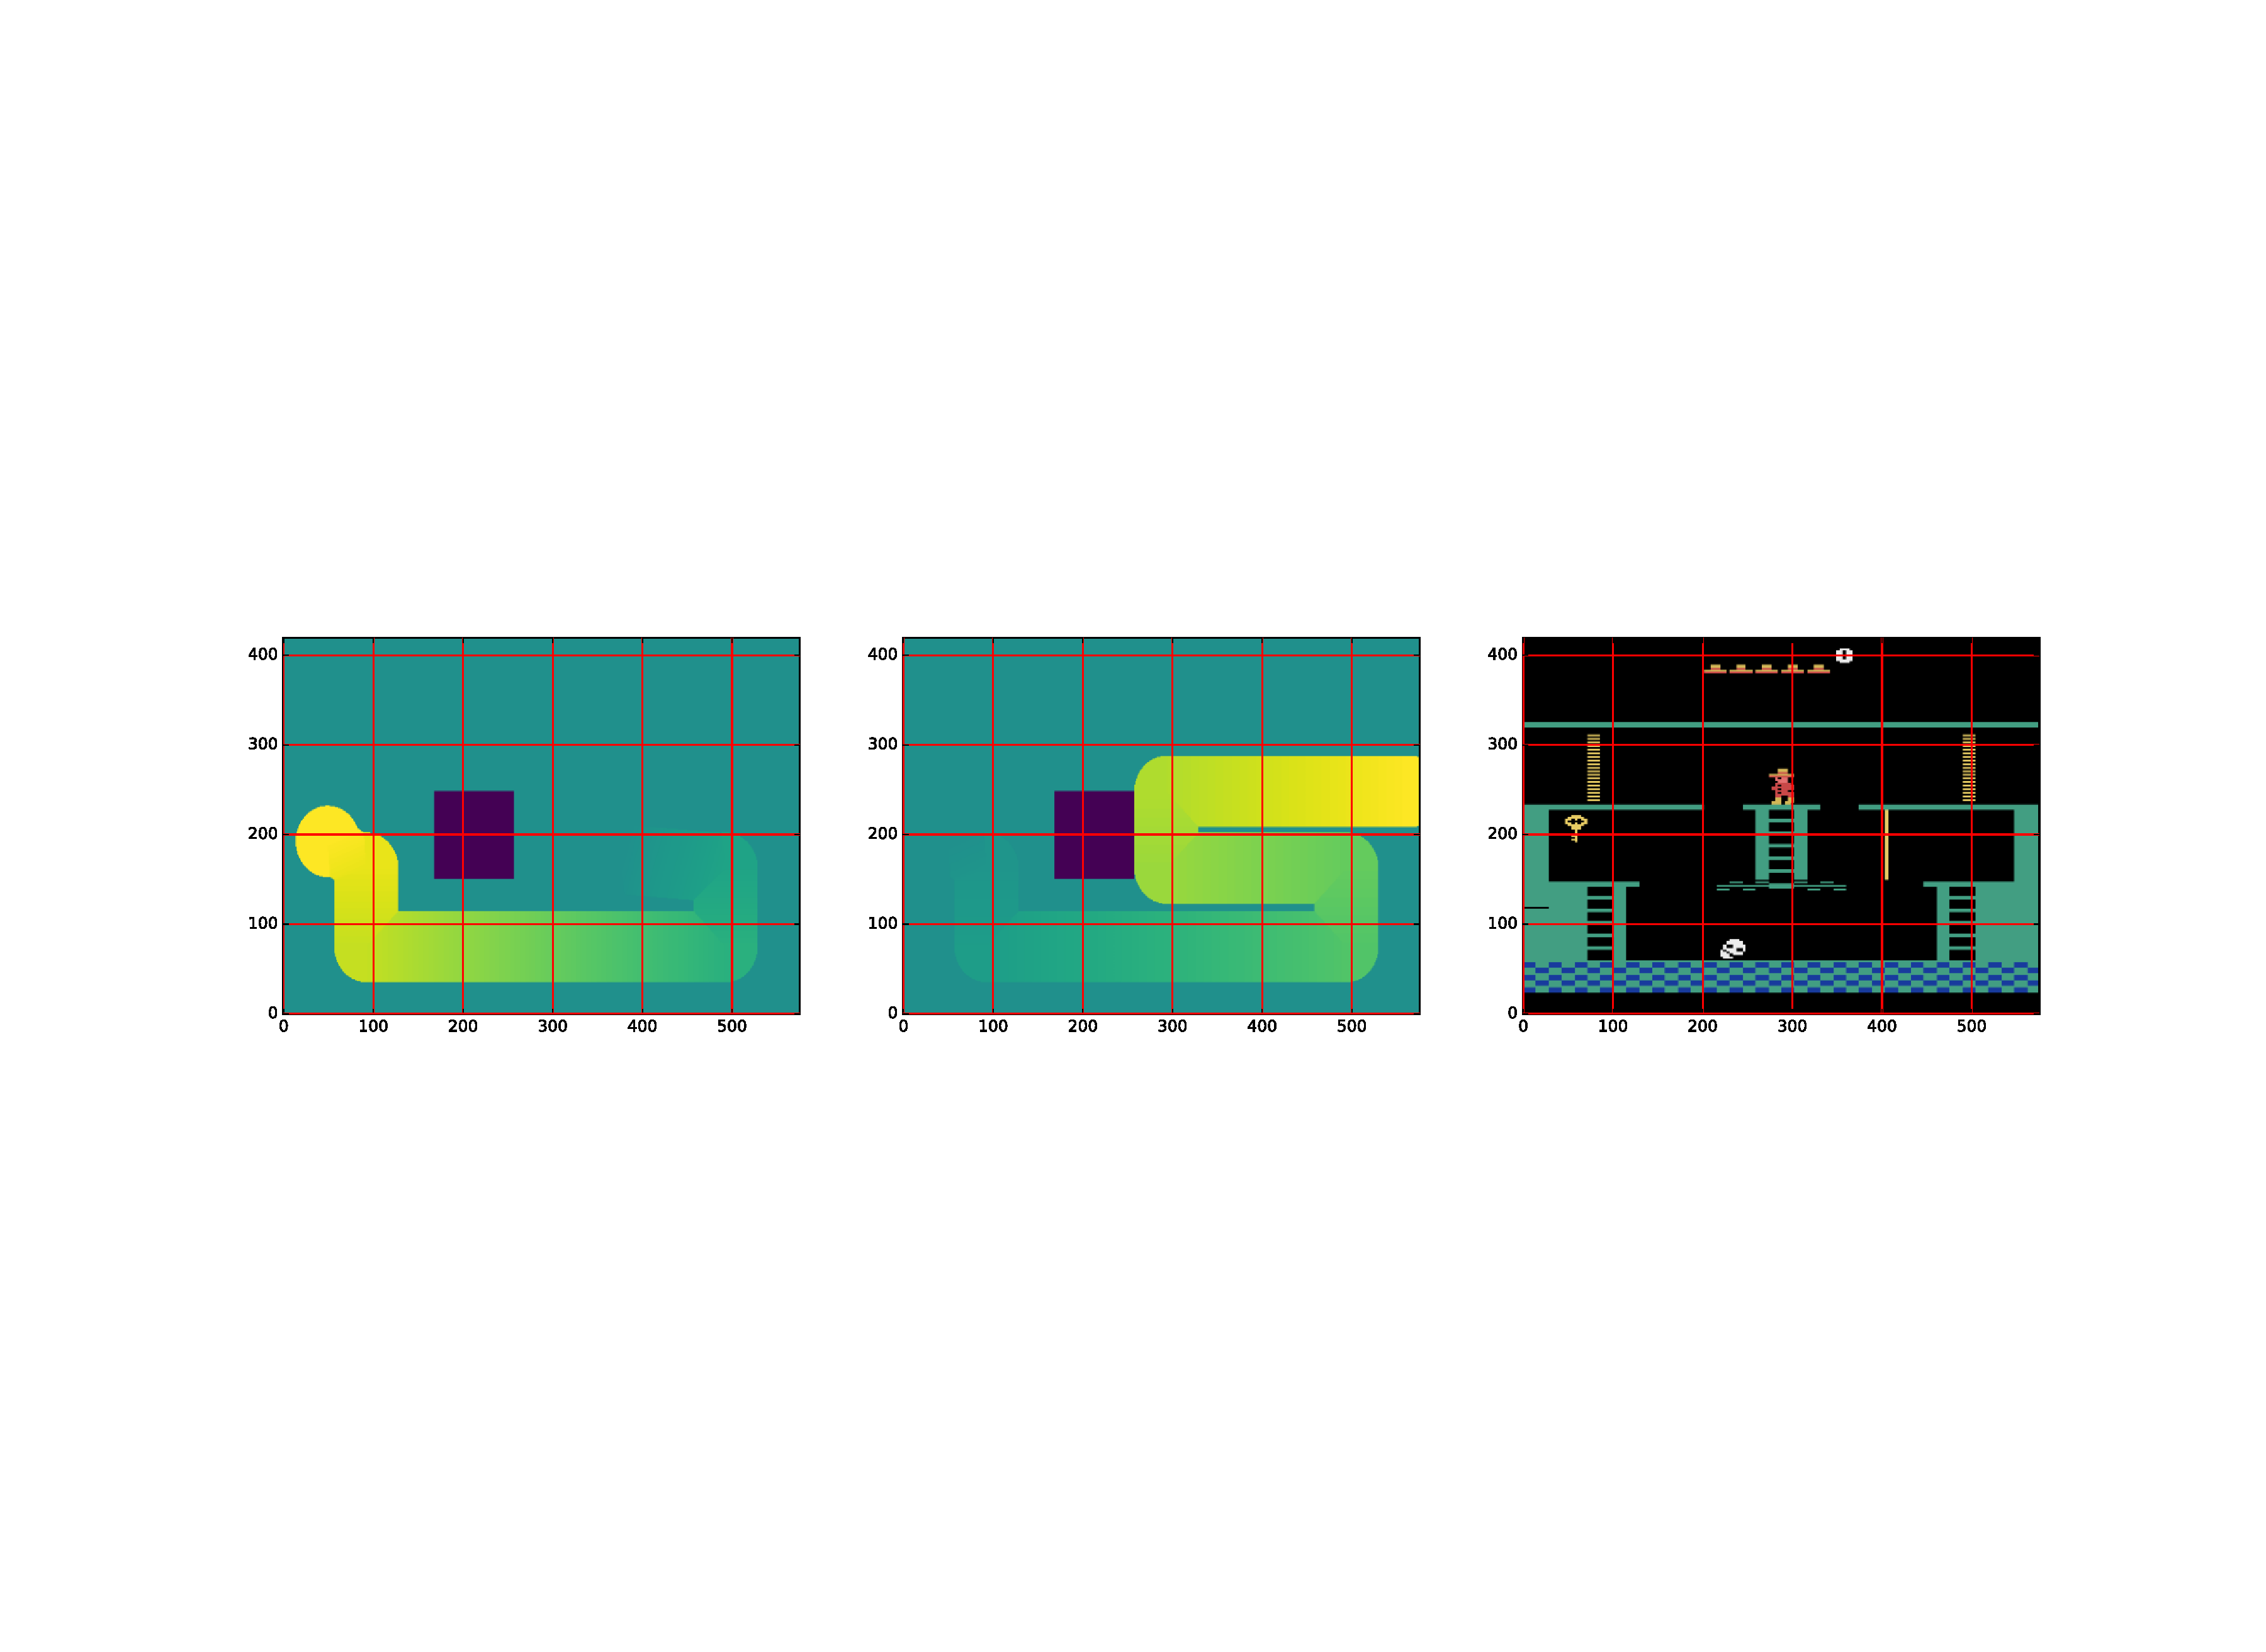
\includegraphics[width=\textwidth]{img/shaping.pdf}
\end{center}
\caption[The potential function $\phi$ field used for shaping]{The potential
  function $\phi$ field used for shaping. From left to right: $v_5=0$, $v_5=1$,
  reference screenshot from the game. Vertical axis is $v_4$, horizontal axis
  is $v_3$. Yellow is $\phi(\cdot)=2$, deep purple is $\phi(\cdot)=1$.\label{fig:shaping}}
\end{figure}
}

\subsection{Options}
We created options to test with \ac{SMDP} Sarsa. We have 8 options, that
correspond to the 8 possible minimal actions.
\begin{itemize}
  \item \textsc{Noop}: Take action \textsc{Noop} during $frame\_skip$ frames.
    Primitive actions in Atari games treated as \ac{SMDP} also last
    $frame\_skip$ frames, so this is just the primitive \textsc{Noop} action.
  \item \textsc{Up}, \textsc{Down}, \textsc{Left}, \textsc{Right}: the normal
    directions are followed until:
    \begin{itemize}
      \item Their coordinate ($y$ for \textsc{Up} and \textsc{Down}, $x$ for the
        rest) stops changing for a long enough time. For example, when Joe bumps
into a wall.
      \item It wasn't possible to move in the other axis when the action started
        and it is possible now, or vice versa. This is implemented by generating
        tentative moves in the other axis every $frame\_skip$ frames, and
        checking if their $x,y$ coordinates are different.
      \item Joe will lose a life or start falling in $n_{\text{backtrack}} \cdot
        frame\_skip$ frames. This is implemented by backtracking generated
        states when these things happen, in a similar manner to function
        \textsc{Obstacle-Wait}, from \ffref{alg:iw-funcs}.
        \begin{itemize}
          \item If the option starts when Joe is already in mid-air, it behaves
            like the \textsc{Noop} option.
        \end{itemize}
    \end{itemize}
  \item \textsc{Fire}, \textsc{LeftFire} and \textsc{RightFire}: Take the
    corresponding action once, then take action \textsc{Noop} until the
    character lands again.
\end{itemize}

It is possible to take these actions at all times, their initiation set,
$\mathcal{I}$, is the set of all states, $\mathcal{S}$.

\section{Planning}
\acl{IW} was first applied to Atari games by \citet{lipovetzky2015classical}.
They used $\textsc{IW}(1)$ only (\ffref{subsec:iterated-width}) in an on-line
setting (\ffref{subsec:online-setting}). Since \ac{IW} operates only on Boolean
variables, they convert each of the \ac{RAM}'s memory positions to 256
variables, one for every possible value of the byte.

We downloaded, read and run their kindly provided
implementation\footnote{\href{https://github.com/miquelramirez/ALE-Atari-Width}{https://github.com/miquelramirez/ALE-Atari-Width}}.
Their agent behaved erratically until it got to the bottom floor, past the skull
or without the skull. Then, it made a beeline for the key.

\subsection{Width of \acl{MR}}
A successful player of \ac{MR} must visit the same location several times. She
needs to take certain paths and backtrack them, to wait for obstacles to cycle
between passable and impassable, to take into account doors that may or may not
be opened and the contents of her inventory.

At least, the path to the solution will involve being at a certain location, for
more than one step of time. Thus, the search algorithm must not prune a state
when the time (as given by, for example, \hyperref[ram:frame]{memory position 0x80})
changes and the position does not.

\newcommand{\ram}[2]{\hyperref[ram:#1]{#2}}

Location of Joe can be represented by the contents of the memory positions
$\langle\text{\hyperref[ram:x]{0xAA}},
\text{\hyperref[ram:y]{0xAB}},
\text{\hyperref[ram:screen]{0x83}}\rangle$,
that is, $x$, $y$, and screen location. This, combined with position
\hyperref[ram:frame]{0x80}, intuitively suggests that \ac{MR} has a \emph{width}
of at least 4.

The authors of \ac{IW} discarded applying a higher width than 1 to Atari games
because the number of tuples to record is too large. We get around this limitation
using domain knowledge: we prune only on the 3-tuple representing location. All
the other memory positions are considered to not change in value. Henceforth, we
will refer to this algorithm as ``\ac{IW}(3)'' or ``\ac{IW}(3) on position'',
even the original \ac{IW}(3) would prune far less often.

\ac{IW}(3) on position prunes a movement when Joe does not move to a different
place. Thus, it allows for exploring the whole screen, while pruning several
redundant moves such as applying different actions while in the middle of a jump.
As shown in \ffref{fig:iw-1-3}, this makes for much better exploration of the
environment.

How is it possible that we can use \ac{IW}(3) on a problem with width $\geq 4$?
The key lies in the on-line setting. Rather than looking for all the paths until
the end, the algorithm only explores to a certain point and then picks an
action. Thus, focusing on spatial exploration works relatively well
(\ffref{sec:score-planning}).
\begin{figure}[hbtp]
\begin{center}
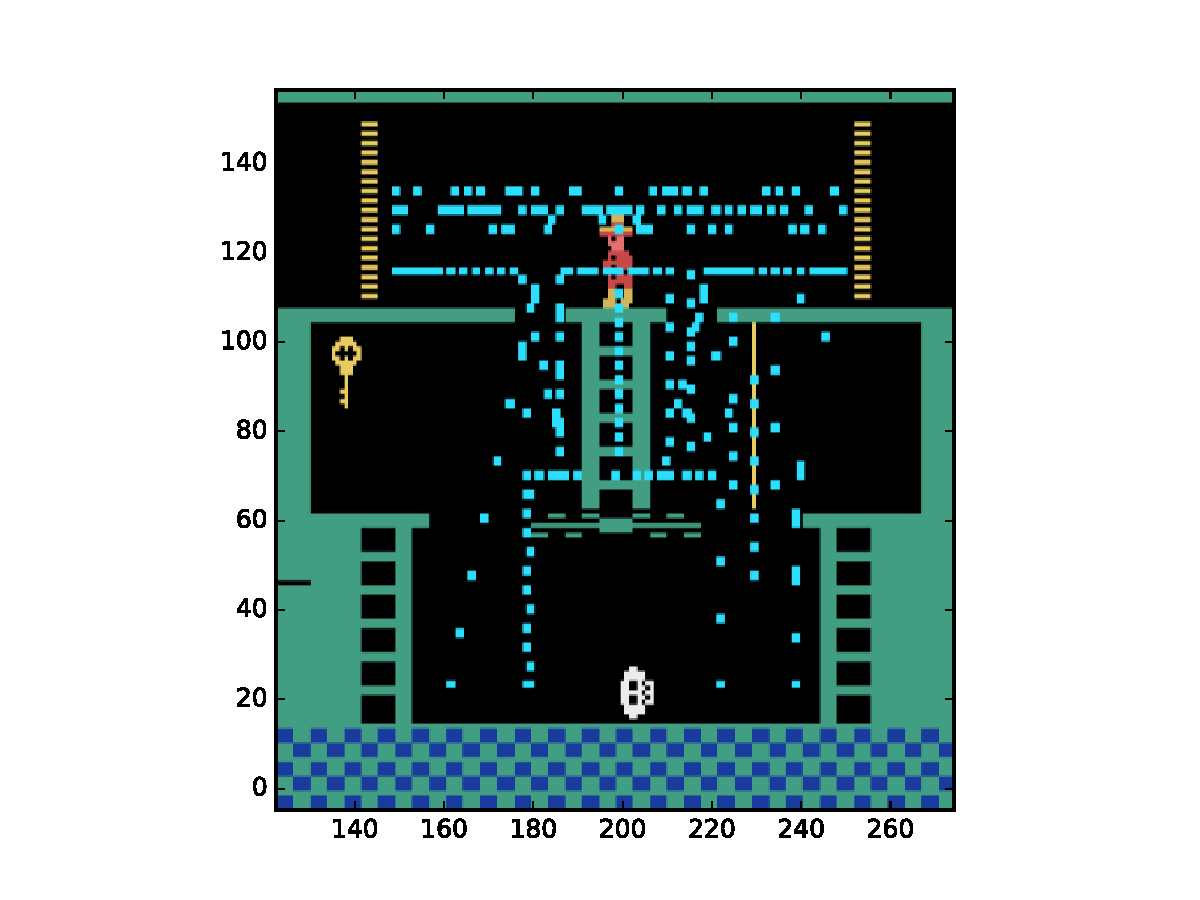
\includegraphics[width=\textwidth / 2 -2cm]{img/iw1-explore-thick.pdf}
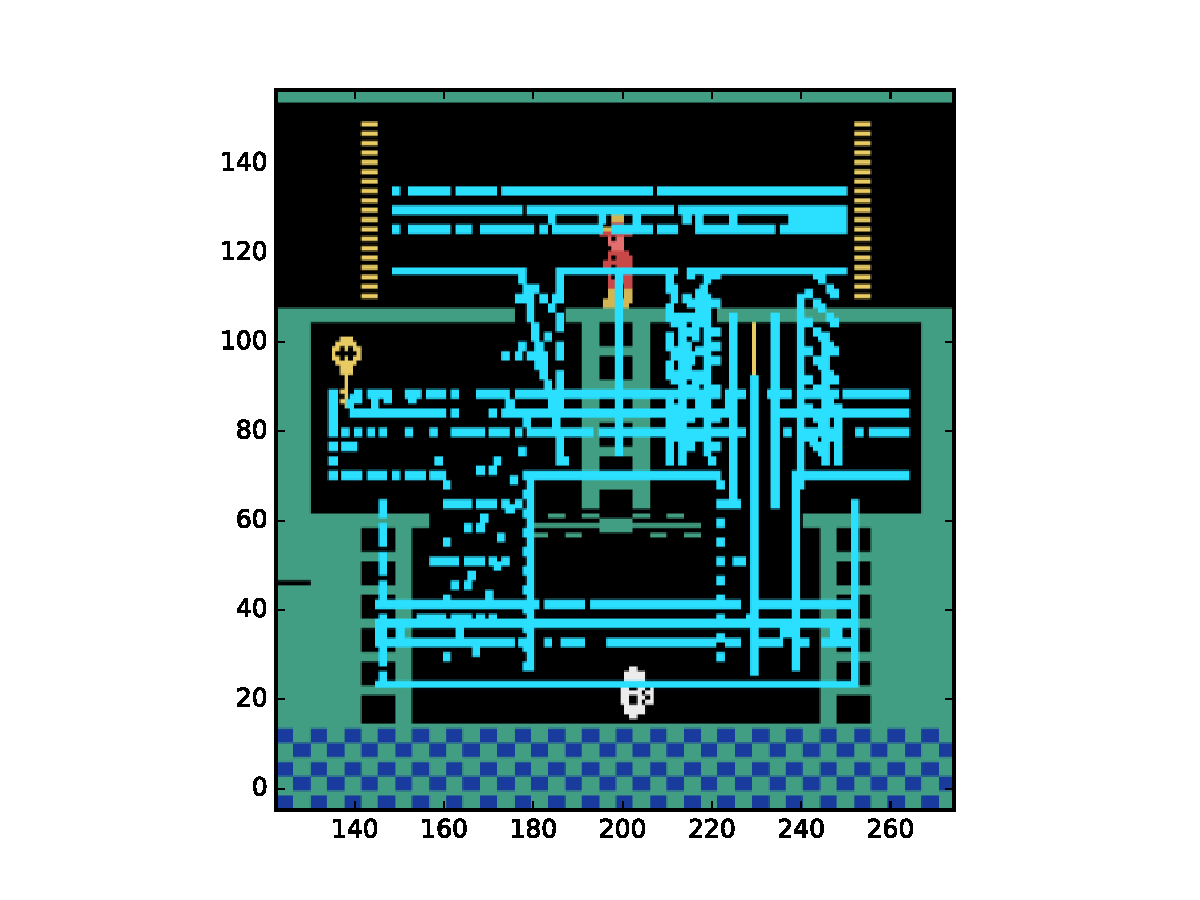
\includegraphics[width=\textwidth / 2 -2cm]{img/iw3-explore-thick.pdf}
\end{center}
\caption[Comparison of exploration in the first screen by $\textsc{IW}(1)$ and
$\textsc{IW}(3)$ on position.]
{Comparison of exploration in the first screen by $\textsc{IW}(1)$ and
$\textsc{IW}(3)$ on position. Observe that $\textsc{IW}(1)$, to the left, prunes
all paths that move to the right-middle platform, since their $y$ coincides with the
the central platform and their $x$ coincides with the right-top platform.
Our restricted $\textsc{IW}(3)$ only prunes for repeated positions, so it has no
problems finding the key.}
\label{fig:iw-1-3}
\end{figure}

\subsection{Improving score with domain knowledge\label{subsec:domain-explanation}}
\subsubsection{Caring about life}
This one is noted and suggested by \citet{lipovetzky2015classical}. Since the
death of Panama Joe does not reduce the score, the algorithm dies often just to
instantly move to a desired location. This would be fine if the agent never lost
a life unintentionally. However, by the nature of its over-pruned planning, this
is not the case.

\ac{IW}, like \ac{BFS} (\ffref{alg:bfs}), has a single \ac{FIFO} queue as
frontier. We add another, low-priority, queue, that is only used when
the first queue is empty. In the low priority queue, we put the nodes where
Panama Joe has lost a life.

The agent still dies unnecessarily sometimes, when the agent has explored first
sequences of actions that lead to reward and death. In some of those
cases, this causes the nonlethal ways to get to the score to be pruned too early.

\subsubsection{Incentivising room exploration}
More often than not, our agent would follow a path of rewards to the bottom
floor of the pyramid (room 20 or 23, \ffref{fig:montezuma-map}), and then be
stuck there, not finding any positive rewards. Thus, we added a small reward
(+1) to exploring new screens.

This created perverse incentives. The agent often enters room 5 from room 6, or
room 17 without having any keys, and then immediately leaves, unable to obtain
more score in there. However, overall, it helps performance.

\subsubsection{Randomly pruning rooms}
In each tree expansion, upon each first visit to a room (except the first one),
that room is pruned with a certain probability. When a room is pruned, we prune
all the nodes that end in that room. On some lucky frames, this makes the agent
explore farther.

On unlucky frames, the agent may find the return of all the actions being zero.
We mitigate this by, after expanding the tree, not just taking the first action
of the branch with highest return, but storing the whole branch. At each frame,
the newly generated branch is compared with the previous one, and the one with
the most return is followed.

\subsubsection{Prioritising long paths}
Ties in branch return are broken by length of the branch. Except for the first
action, where ties are broken uniformly randomly.

\subsubsection{Overriding pruning near timed obstacles}
The basic intuition is: when losing a life because of running into an obstacle
that will disappear after some time, wait.

In practice, this means:
\begin{itemize}
  \item Lose a life after walking into the obstacle, not jumping.
  \item Backtrack to a position ``outside'' the obstacle, that allows you to
    survive until the same time instant.
  \item Wait until the obstacle goes away, by testing moves into the direction
    of the direction you backtracked from, or a maximum time to wait.
  \item Add the resulting node to the frontier.
\end{itemize}

\subsubsection{Preventing short-sighted door opening}
A fundamental shortcoming of our agent is that it opens doors not to explore
what is behind them, but because doing so increments the score. As a consequence
of this (and of shortsightedness), it opens both the doors in each screen 1 and
5, rendering the game impossible to complete (as explained in
\ffref{subsec:mr-description}). We penalised this behaviour by giving a penalty
to opening the wrong doors ($-10\,000$).

\subsection{Implementation\label{subsec:implementation-iw}}
Our agent is described in
Algorithms~\ref{alg:iw-funcs},~\ref{alg:iw-optimised}~and~\ref{alg:online-setting}.
\textsc{Online-Setting-Episode} in \ffref{alg:online-setting} is the entry
point.

Each time step, we reuse the search tree created in the last time step.
Emulating frames is the most computationally expensive step in the search, so we
restrict each time step to emulating $max_{ef}$ frames
\citep{lipovetzky2015classical}.

As an efficiency improvement, we can take several actions of the planned
sequence before re-calculating the search tree. Since our algorithm is neither
optimal nor complete, this may degrade or enhance performance.

$s[i]$ is used to denote the \ac{RAM} position $i$ in node $s$. When a node $s$ is
created from the transition function $f$, $s.\textsc{Return}$ contains the
reward accumulated while emulating the action in $s$.

The transition function $s' = f(s, a)$ is implemented in the \ac{ALE} by first
loading the state $s$ to the emulator, then applying action $a$ for $frame\_skip$
frames. In the end we observe the resulting state $s'$, with its reward. The
$frame\_skip$ constant is very commonly used for playing Atari games, since the
state changes little every frame (\cite{bellemare2013arcade},
\cite{lipovetzky2015classical}, \cite{mnih2015human},
\cite{kulkarni2016hierarchical}, \dots).

\textsc{Noop}, \textsc{Left}, \textsc{Right}, \textsc{Up} and \textsc{Down} are
actions the character can take, corresponding to standing still and moving
in a certain direction without jumping, respectively.

\begin{algorithm}[hbtp]
\newcommand{\n}[1]{0x#1}
\newcommand{\tn}[1]{\text{0x#1}}
\renewcommand{\r}[1]{ram[\text{0x#1}]}
\begin{algorithmic}
\Procedure{Online-Setting-Episode}{}
\State Initialise action and return 1-based-index sequences,
$a \gets []$, $R \gets []$
\State $n_a$: number of actions to take without re-planning
\State $p_r$: probability that a room is pruned
\State $f$ is the emulation function
\State $max_{ef}$ maximum number of frames to emulate per search
\State $max\_wait$: max. n. of actions to wait for an obstacle to become passable
\State $max\_backtrack$: max. n. of nodes to backtrack when running into an obstacle
  \Repeat
    \State Observe state $s$.
    \State $s.\textsc{Return} \gets 0$
    \State $(a', R') \gets \Call{IW3}{\langle s, \mathcal{A}, f \rangle,
      max_{ef}, max\_wait, max\_backtrack, p_r}$
    \If{$R=[] \vee R'[1] > R[1]$}
      \State $R \gets R', a \gets a'$
    \EndIf
    \For{$i$ from 1 to $\min(n_a, \Call{Length}{R})$}
      \State Take action $a[i]$, observe and tally reward
    \EndFor
    \State $R \gets R'[n_a+1,n_a+2,\dots]$, $a \gets a'[n_a+1,\dots]$
   \Until{the game is over}
\EndProcedure
\Function{Branch-Return}{$s$}
\State \textbf{if} $s$ is a leaf node and has opened a wrong door,
$s.\textsc{Return} \gets -10\,000$ \textbf{end~if}
\State \textbf{if} $s$ is a leaf node \Return $[s.\textsc{Return}]$ \textbf{end~if}
\State $r_s = \Call{Branch-Return}{c} \, \forall c \in s.\textsc{Children}$
\State $r \gets \max_{r\in r_s} r$, comparing by first element, ties broken by
higher length.
\State \Return $\Call{Append}{[s.\textsc{Return}], \gamma \cdot r}$
\EndFunction
\end{algorithmic}
\caption{The agent in an on-line setting, using \ac{IW}(3) for \acl{MR}, along
with some supporting functions for \ac{IW}(3).}
\label{alg:online-setting}
\end{algorithm}

\begin{algorithm}[hbtp]
\newcommand{\n}[1]{0x#1}
\newcommand{\tn}[1]{\text{0x#1}}
\renewcommand{\r}[1]{ram[\text{0x#1}]}
\begin{algorithmic}
\Function{Update-Novelty}{$seen\_tuples, visited\_screens, pruned\_screens, ram,
  p_r$}
\If{$\neg visited\_screens[\r{83}]$}
\State $visited\_screens[\r{83}] \gets true$
\State With probability $p_r$: $pruned\_screens[\r{83}] \gets true$
\EndIf
\State $seen\_tuples[ \langle \r{AA},\r{AB},\r{83} \rangle ] \gets true$
\EndFunction
\Function{Check-Novelty}{$seen\_tuples, pruned\_screens, ram$}
\State \Return $\neg (pruned\_screens[\r{83}] \, \vee $
\State \hspace{3cm} $seen\_tuples[ \langle \r{AA},\r{AB},\r{83} \rangle ])$
\EndFunction
\Function{On-Ground?}{$ram$}
\State \Return $\r{D6}=\tn{FF} \wedge \r{D8} =0$
\EndFunction
\Function{Falling?}{$ram$}
\State \Return $\r{D8} \neq 0$
\EndFunction
\Function{LRUD?}{$a$}
\State \Return Whether the action $a \in \{ \textsc{Left},\textsc{Right}, \textsc{Up},
\textsc{Down} \}$. 
\EndFunction
\Function{Obstacle-Wait}{$f, obstacle\_child, q, max\_wait, max\_backtrack$}
  \State $p \gets obstacle\_child.\textsc{Parent}$, $p_p \gets obstacle\_child$,
    $l_0 \gets p[\tn{BA}]$
  \For{$i \in [0,max\_backtrack)$}
    \State $f^i(s, a) = f(f(\dots f(s, a) \dots, a), a)$, totalling $i+1$ applications of $f$
    \State $n \gets f^i(p, \textsc{Noop})$
    \If{$\Call{On-Ground?}{n} \wedge n[\tn{BA}] = l_0$}
      \For{$i \in [0,max\_wait)$}
        \State $n_{\text{test}} \gets f^2(n, p_p.\textsc{Action})$
        \If{$\Call{On-Ground?}{n_{\text{test}}} \wedge n_{\text{test}}[\tn{BA}] = l_0$}
        \State \Return $\Call{Queue-Insert}{q, n}$
        \EndIf
        \State $n \gets f(n, \textsc{Noop})$
      \EndFor
    \EndIf
    \State $p_p \gets p$, $p \gets p.\textsc{Parent}$
  \EndFor
  \State \Return $q$
\EndFunction
\end{algorithmic}
\caption{Supporting functions for \ac{IW}(3) (\ffref{alg:iw-optimised})}
\label{alg:iw-funcs}
\end{algorithm}

\begin{algorithm}[hbtp]
\newcommand{\n}[1]{0x#1}
\newcommand{\tn}[1]{\text{0x#1}}
\renewcommand{\r}[1]{ram[\text{0x#1}]}
\begin{algorithmic}
\Function{IW3}{$problem=\langle s_0, \mathcal{A}, f \rangle, max_{ef},
  max\_wait, max\_backtrack, p_r$}
  \State $seen\_tuples \gets false$ for all tuples $[0,256)^2 \times [0,24)$
  \State $visited\_screens[i] \gets false,\,pruned\_screens[i] \gets false,\,
  \forall i\in[0,24)$
  \State $visited\_screens[s_0.\r{83}] \gets true$
  \State $q \gets [s_0]$, $q_l \gets []$, \ac{FIFO} queues representing the frontier
  \While{$\neg \Call{Empty?}{q} \wedge \neg \Call{Empty?}{q_l} \wedge
          \text{num.~emulated~frames} < max_{ef}$}
    \State Get $s \gets \Call{Pop}{q}$, or $\Call{Pop}{q_l}$ if $q$ is empty.
    \State $obstacle\_child \gets \varnothing$
    \For{\textbf{each} child $c = f(s, a) \, \forall a \in \mathcal{A}$}
    \If{$\Call{Check-Novelty}{seen\_tuples, pruned\_screens, c}$}
    \State $\Call{Update-Novelty}{seen\_tuples, visited\_screens,
      pruned\_screens, c, p_r}$
    \If{$c[\tn{BA}] < s[\tn{BA}]$, this node loses a life} 
      \If{$\Call{On-Ground?}{c} \wedge \Call{On-Ground?}{s}
        \wedge \Call{LRUD?}{a}$}
        \State $obstacle\_child \gets c$
      \EndIf
      \State $q_l \gets \Call{Queue-Insert}{q_l, c}$
    \Else
    \If{$\Call{Falling?}{c} \wedge \Call{On-Ground?}{s}
        \wedge \Call{LRUD?}{a}$}
        \State $obstacle\_child \gets c$
        \State \textbf{if} $a=\textsc{Down}$ \textbf{then} $q \gets
        \Call{Queue-Insert}{q, c}$ \textbf{end~if}
      \Else
        \State $q \gets \Call{Queue-Insert}{q, c}$
      \EndIf
    \EndIf
    \EndIf
    \EndFor
    \If{$obstacle\_child \neq \varnothing$}
    \State $q, \gets \Call{Obstacle-Wait}{f, obstacle\_child, q,
max\_wait, max\_backtrack$}
    \EndIf
  \EndWhile
  \State \Return $\Call{Branch-Return}{s_0}$
\EndFunction
\end{algorithmic}
\caption{\ac{IW}(3) for \acl{MR}, optimised with domain knowledge}
\label{alg:iw-optimised}
\end{algorithm}

% The learning in tabular case took 26h
% The learning in NN so far taking 13h
% IW so far taking 13h

%%% Local Variables: 
%%% mode: latex
%%% TeX-master: "../report"
%%% End: 
